% Original book p65; original base PDF p69; input PDF p90; p065_s01 一、1
% Role: question; original field: diagrams[0].tikz
% Compile with XeLaTeX from this figures/ directory.
\documentclass[12pt,tikz,border=5pt]{standalone}
\usepackage{fontspec}
\setmainfont[Path=../fonts/]{DroidSansFallback.ttf}
\setsansfont[Path=../fonts/]{DroidSansFallback.ttf}
\usepackage{amsmath,amssymb}
\usepackage{tikz}
\usetikzlibrary{calc,angles,quotes,arrows.meta,decorations.pathreplacing,decorations.pathmorphing,decorations.markings,patterns,positioning,fit,backgrounds,matrix,intersections,shapes.geometric}
\begin{document}
\color{black}
\tikzset{every picture/.append style={color=black}}
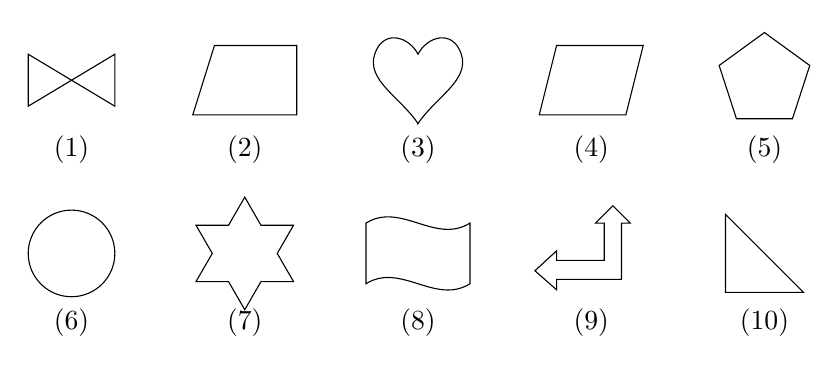
\begin{tikzpicture}[scale=1.1]\begin{scope}[shift={(0,2)}]\draw (-.5,-.3)--(.5,.3)--(.5,-.3)--(-.5,.3)--cycle;\node at (0,-.8){(1)};\end{scope}\begin{scope}[shift={(2,2)}]\draw (-.6,-.4)--(.6,-.4)--(.6,.4)--(-.35,.4)--cycle;\node at (0,-.8){(2)};\end{scope}\begin{scope}[shift={(4,2)}]\draw (0,-.5)..controls(-.2,-.2)and(-.6,0)..(-.5,.3)..controls(-.4,.6)and(-.1,.5)..(0,.3)..controls(.1,.5)and(.4,.6)..(.5,.3)..controls(.6,0)and(.2,-.2)..cycle;\node at (0,-.8){(3)};\end{scope}\begin{scope}[shift={(6,2)}]\draw (-.6,-.4)--(.4,-.4)--(.6,.4)--(-.4,.4)--cycle;\node at (0,-.8){(4)};\end{scope}\begin{scope}[shift={(8,2)}]\draw (90:.55)--(162:.55)--(234:.55)--(306:.55)--(18:.55)--cycle;\node at (0,-.8){(5)};\end{scope}\begin{scope}[shift={(0,0)}]\draw (0,0) circle(.5);\node at (0,-.8){(6)};\end{scope}\begin{scope}[shift={(2,0)}]\draw (90:.65)\foreach \a in {120,150,...,420}{--(\a:{ifthenelse(mod((\a-90)/30,2)==1,.375,.65)})}--cycle;\node at (0,-.8){(7)};\end{scope}\begin{scope}[shift={(4,0)}]\draw (-.6,-.35)..controls(-.2,-.1)and(.2,-.6)..(.6,-.35)--(.6,.35)..controls(.2,.1)and(-.2,.6)..(-.6,.35)--cycle;\node at (0,-.8){(8)};\end{scope}\begin{scope}[shift={(6,0)}]\draw (-.65,-.2)--(-.4,.03)--(-.4,-.08)--(.15,-.08)--(.15,.35)--(.05,.35)--(.25,.55)--(.45,.35)--(.35,.35)--(.35,-.3)--(-.4,-.3)--(-.4,-.42)--cycle;\node at (0,-.8){(9)};\end{scope}\begin{scope}[shift={(8,0)}]\draw (-.45,-.45)--(.45,-.45)--(-.45,.45)--cycle;\node at (0,-.8){(10)};\end{scope}\end{tikzpicture}

\end{document}
